% Resumo simples das cinco variáveis, para as orientadoras.
% Compila com pdflatex e bibtex (Overleaf).
\documentclass[11pt,a4paper]{article}

\usepackage{iftex}
\ifPDFTeX
  \usepackage[utf8]{inputenc}
  \usepackage[T1]{fontenc}
  \usepackage{lmodern}
\else
  \usepackage{fontspec}
\fi
\usepackage[brazilian]{babel}
\usepackage[a4paper,margin=2cm]{geometry}
\usepackage{graphicx}
\usepackage{float}  % [H] deixa cada figura exatamente onde aparece no texto
\usepackage{enumitem}
\usepackage[font=small,labelfont=bf,labelsep=period]{caption}
\usepackage[colorlinks=true,citecolor=blue,linkcolor=blue,urlcolor=blue]{hyperref}  % citação vira link azul
\usepackage[alf]{abntex2cite}  % citações no padrão ABNT, com \citeonline

\graphicspath{{figuras/}}
\setlist{itemsep=3pt,topsep=3pt}
\setlength{\parskip}{6pt}
\setlength{\parindent}{0pt}
\pagestyle{empty}

\begin{document}

{\Large\bfseries Onde há pistas para prever o mês seguinte?}\\[2pt]
{\large Memória e El Niño nas cinco variáveis do projeto, no Sudeste da América do Sul}\\[4pt]
Emanuel Pinto Sampaio \quad·\quad Novembro de 2026

\section*{A ideia}

Antes de treinar qualquer modelo de previsão, quis saber onde existe alguma pista para prever o mês seguinte em cada uma das cinco variáveis do projeto, que são temperatura do ar, precipitação, umidade específica, pressão e vento. Olhei duas pistas simples.

\begin{itemize}
\item \textbf{Memória.} Quando um mês fica acima do normal, o mês seguinte também tende a ficar?
\item \textbf{El Niño.} O aquecimento do Oceano Pacífico em um mês diz algo sobre o mês seguinte aqui?
\end{itemize}

Usei os dados mensais do ERA5 de 1979 a 2025. O ERA5 é uma base de dados que reconstrói o clima do passado, mês a mês, em todo o planeta. A região é a mesma da iniciação científica de \citeonline{duarte2026previsao} e aparece na Figura 1.

\begin{figure}[H]
\centering
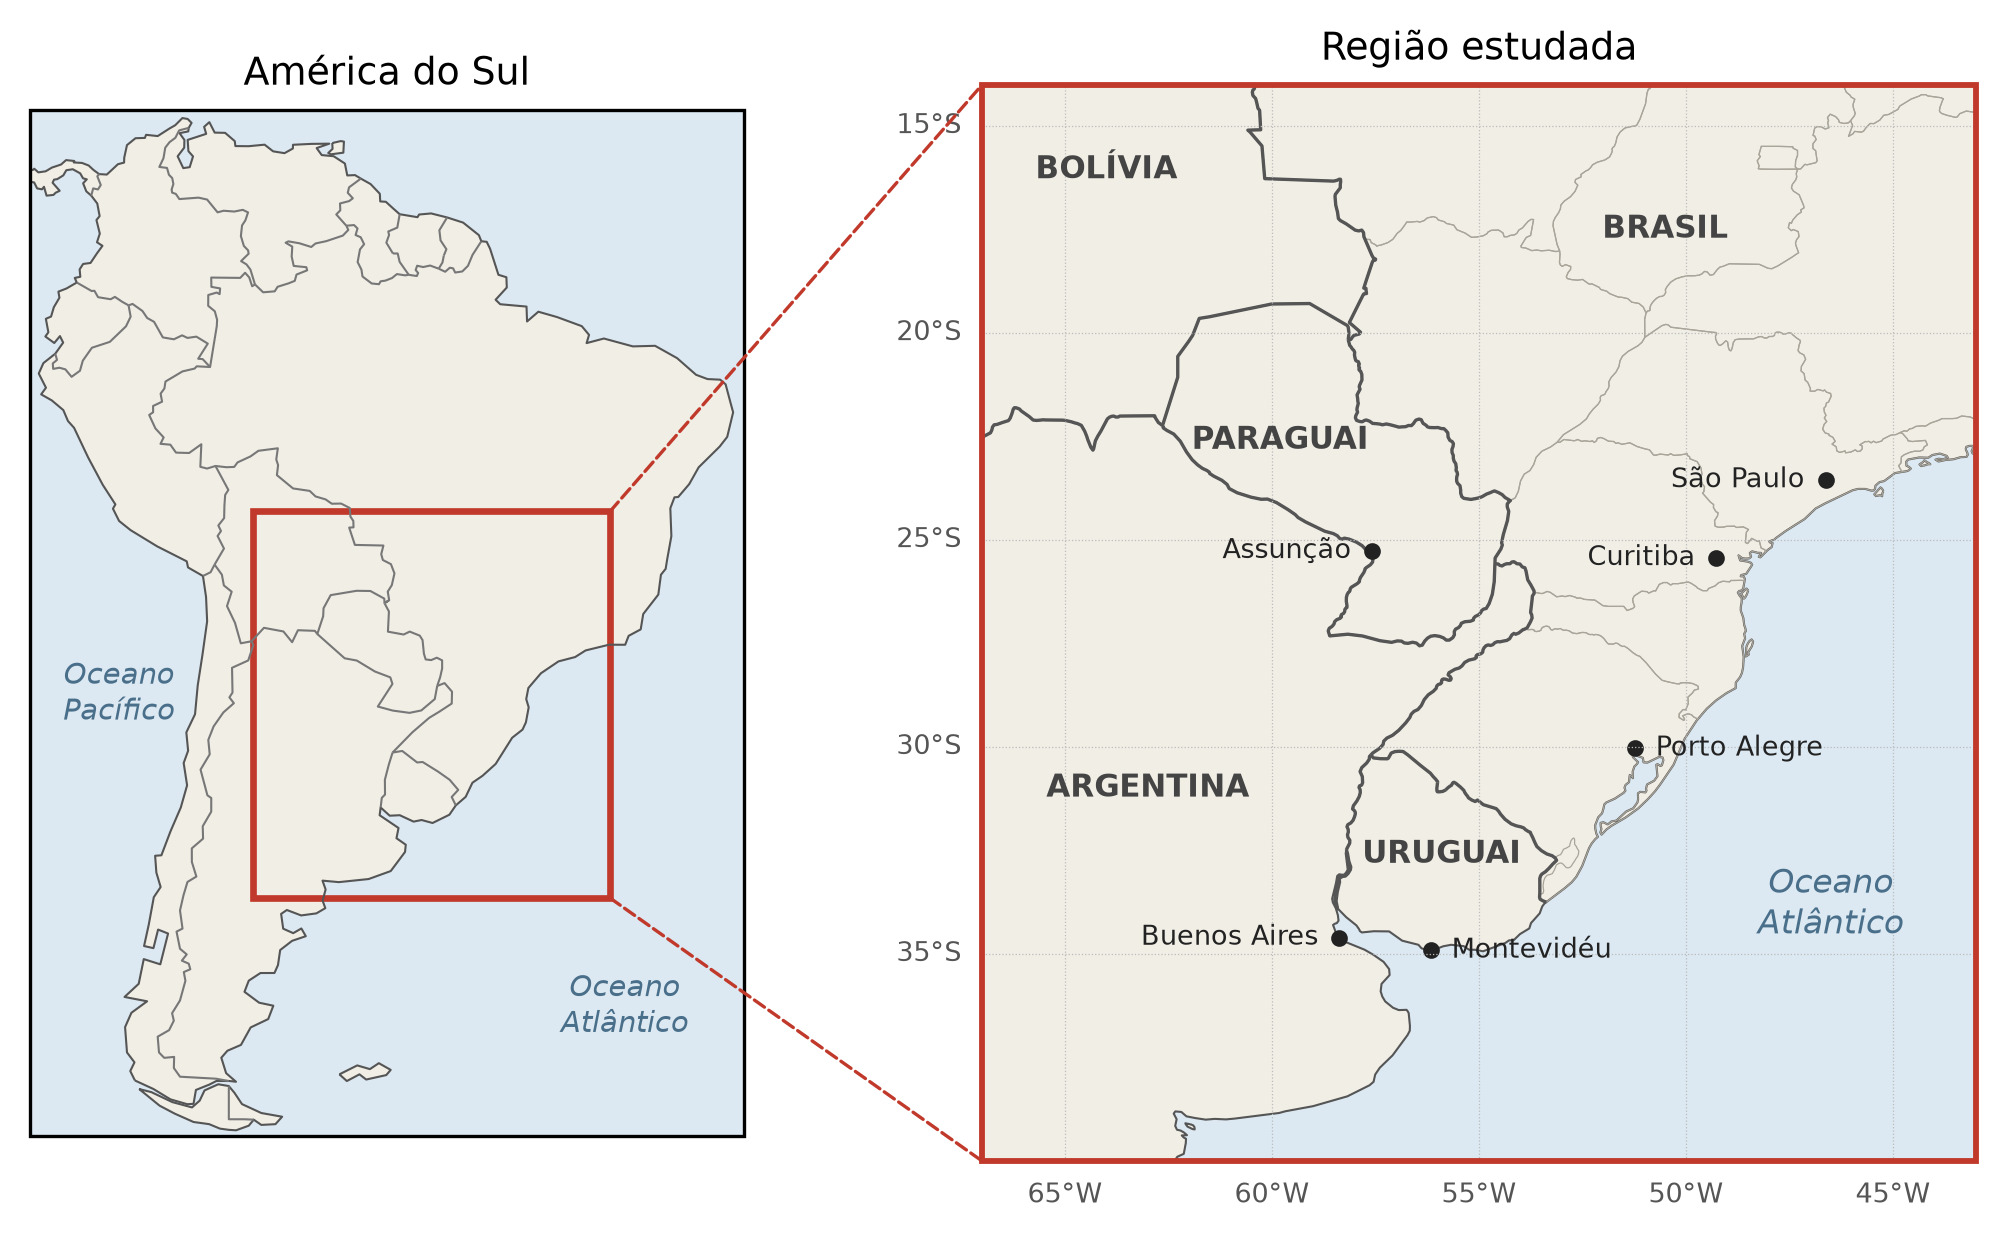
\includegraphics[width=0.85\textwidth]{mapa_regiao.png}
\caption{À esquerda, a América do Sul. À direita, o zoom da região estudada, que cobre o Sul e o Sudeste do Brasil, o Paraguai, o Uruguai e o norte da Argentina.}
\end{figure}

\section*{O que encontrei}

A Figura 2 mostra o resultado em mapas. Na linha de cima está a memória e na de baixo, o El Niño. Quanto mais forte a cor, mais forte a pista. As áreas em branco são aquelas em que o resultado pode ter sido só acaso.

\begin{figure}[H]
\centering
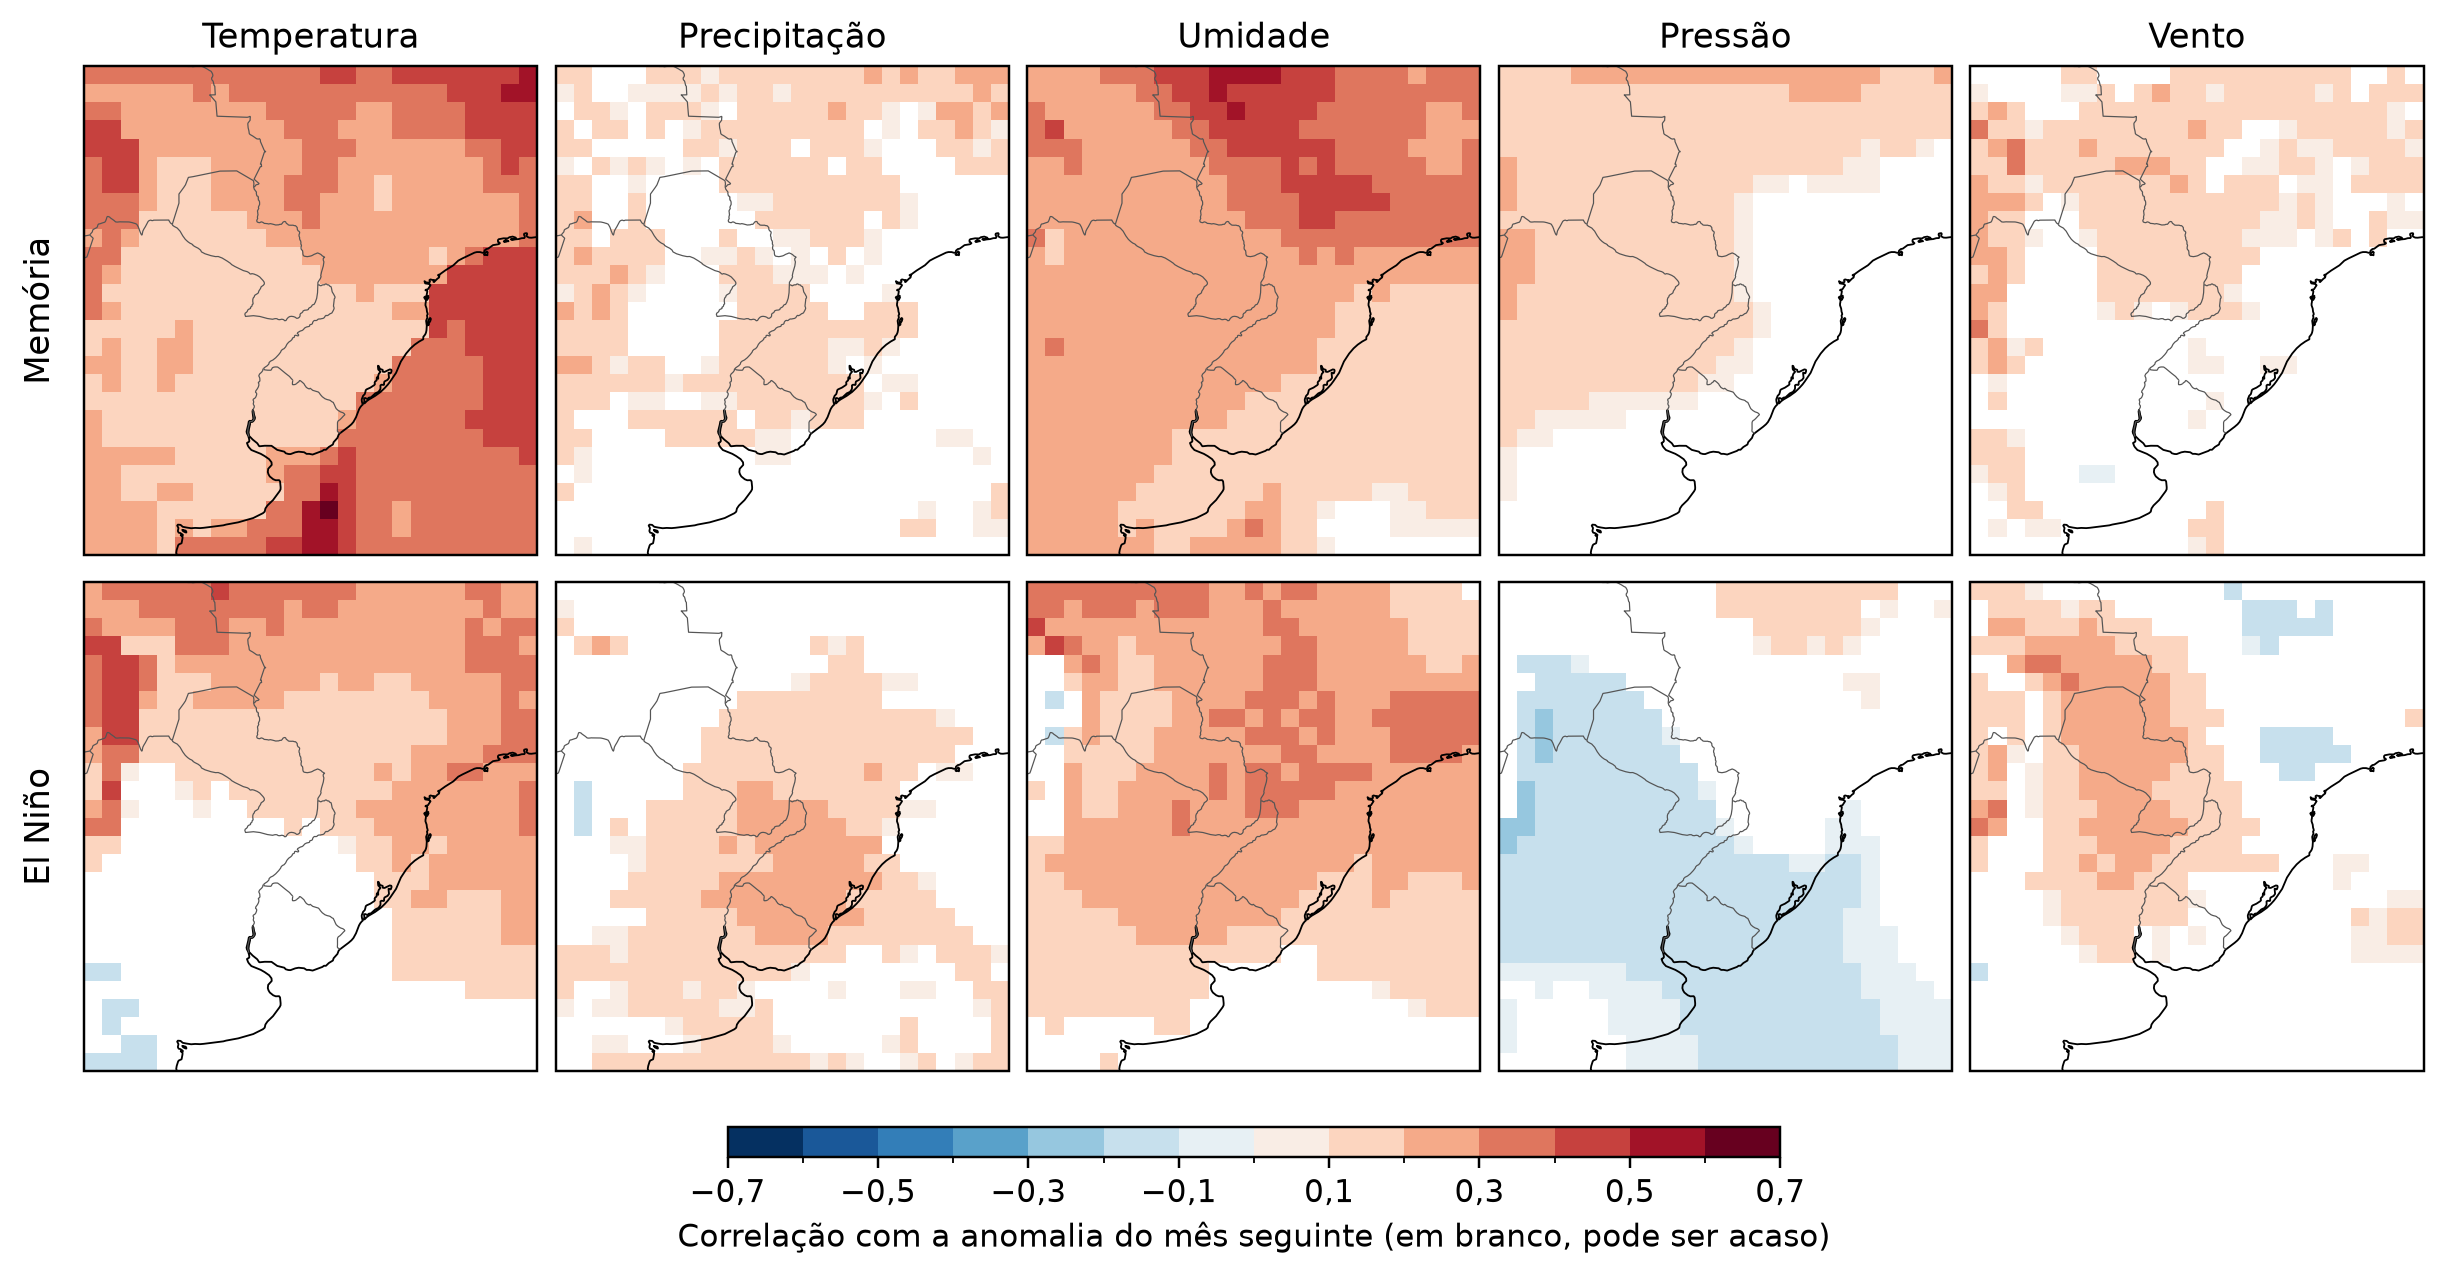
\includegraphics[width=0.92\textwidth]{cinco_variaveis.png}
\caption{Em cima, a memória de cada variável. Vermelho quer dizer que o mês seguinte tende a repetir o mês atual. Embaixo, a pista do El Niño. Vermelho quer dizer que, depois de um El Niño, a variável tende a ficar acima do normal, e azul, abaixo do normal.}
\end{figure}

A \textbf{temperatura do ar} é a variável com mais memória, principalmente sobre o oceano. Isso faz sentido, porque a água demora mais que a terra para esquentar e para esfriar.

A \textbf{umidade específica} faz o contrário e lembra mais sobre o continente, principalmente no Centro-Oeste. Uma explicação possível é a umidade do solo, que muda devagar, mas isso eu ainda não testei.

A \textbf{precipitação} quase não tem memória, porque depende de eventos rápidos, como a passagem de frentes frias. Mesmo assim, o El Niño ajuda a prever a precipitação em metade da região. Depois de um El Niño, ela fica acima do normal no Sul do Brasil, no Uruguai e no nordeste da Argentina, como já se sabia.

A \textbf{pressão} e o \textbf{vento} também têm pouca memória. Sobre o oceano, o vento não tem memória nenhuma, o que pode ajudar a entender por que a rede neural usada por \citeonline{duarte2026previsao} errou mais ali.

No geral, as pistas existem, mas são fracas, o que é normal para previsões de um mês. Depois da temperatura do ar, a umidade específica parece a variável mais promissora para o projeto, porque também tem as duas pistas.

\bibliography{cinco_variaveis}

\end{document}
